\documentclass{beamer}
\usepackage{graphicx} %The mode "LaTeX => PDF" allows the following formats: .jpg  .png  .pdf  .mps
\graphicspath{{./images/}} %Where the figures folder is located
\usepackage{media9}
\addmediapath{./videos/}
\usepackage{animate}
\usepackage{hyperref}
\usepackage{subcaption}
\usepackage{amsmath}
\usepackage{multicol}
\usepackage{paracol}
\usepackage[latin1]{inputenc}
\usetheme{fel}
\usepackage[scaled=0.45]{helvet}

\title{}

\author[]{}
\date[]{}

\institute[]{} 
\begin{document}

\newcommand{\bs}[1]{\LARGE \textit{\textbf{#1}}}


\section{Data reuse in hp-adaptivity}


\subsection{Background}


\begin{frame}

\begin{itemize}
\item Engineers are highly interested in \textbf{extrema} (areas with potential over-heating, wire-melting, structural damage etc.).
\item \vspace{-3mm} \textbf{Extrema} appear in our solutions in forms of \textbf{ingularities, steep gradients, boundary layers}.
\end{itemize}
\vspace{-1mm}
\begin{center}
	\begin{figure}[h!]
	\centering
	\begin{subfigure}{.45\textwidth}
		\centering
		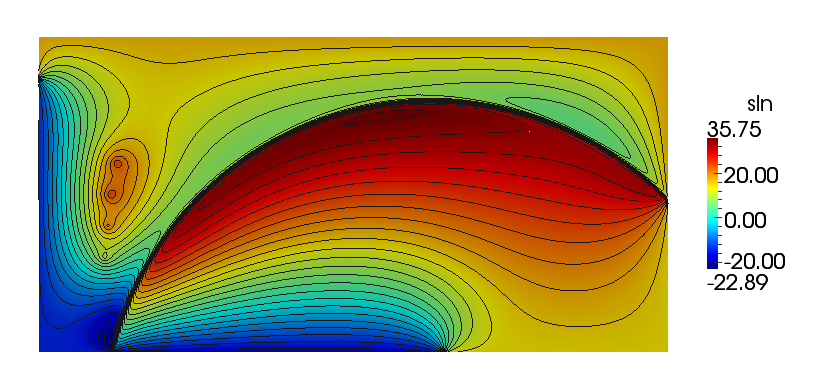
\includegraphics[width=\textwidth]{80-sln.png}
		\vspace{-3mm}
		\caption{Exact solution}
	\end{subfigure}
	\begin{subfigure}{.45\textwidth}
		\centering
		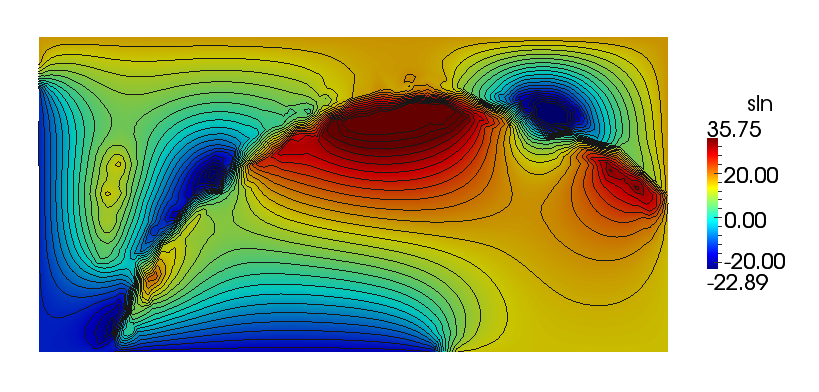
\includegraphics[width=\textwidth]{0-sln.png}
		\vspace{-3mm}
		\caption{Numerical solution with random mesh}	
	\end{subfigure}
	\end{figure}
\end{center}

\vspace{-3mm} 
\begin{itemize}
\item If we only used a single mesh, it is difficult to be sure that we captured all these phenomena.
\item \vspace{-3mm} To be more sure, we can use an overly fine mesh, but doing so, we would waste time, and it may not fit in the memory.
\item \vspace{-3mm} This is because we would have unnecessarily fine mesh in areas where the solution is very well-behaved.
\end{itemize}

\end{frame}

\subsection{Motivation \& Objectives}

\begin{frame}


\begin{center}
	\begin{figure}[h!]
			\centering
			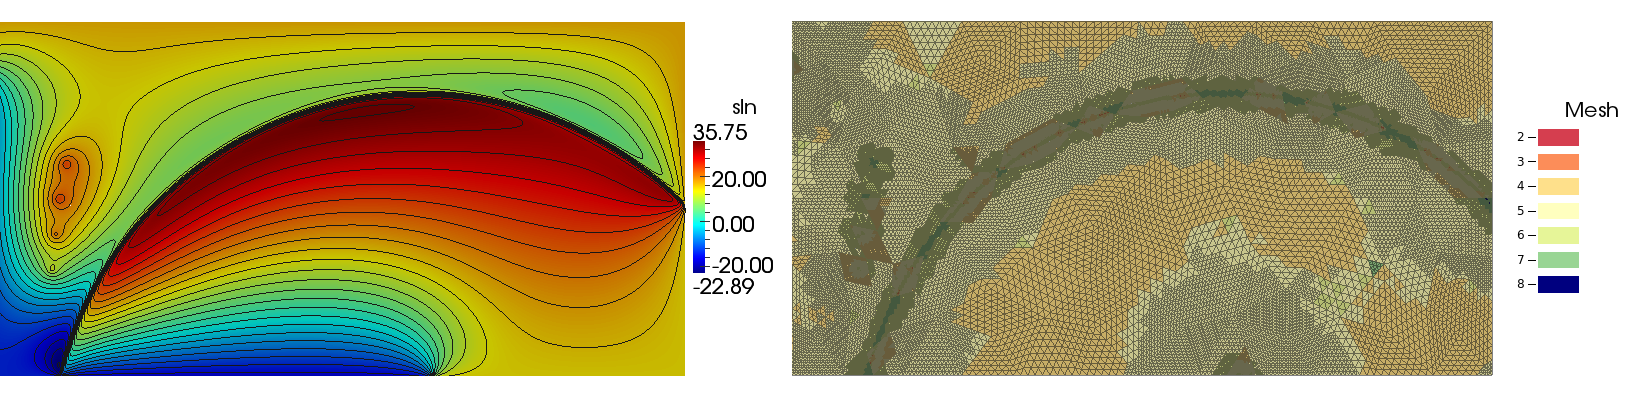
\includegraphics[width=.8\textwidth]{final.png}
			\caption{hp-FEM solution (left) and the final mesh (right)}	
	\end{figure}
\end{center}

\vspace{-5mm} 
{\large We want to save both time \& memory in solving of this problem}

\vspace{-2mm} 
\begin{itemize}
\item To achieve this, we would like to \textbf{quickly} find a mesh good enough to capture the solution with \textbf{as few unknowns as possible}.
\item \vspace{-1mm} The easier part is to save the memory: by cutting down the number of DOFs, we decrease the matrix size
\begin{itemize}
\item \vspace{-2mm} Omitting now potentially higher memory demands for algebraic solver introduced by irregular mesh.
\end{itemize}
\item \vspace{-1mm} The difficult path is to save the time:
\begin{itemize}
\item \vspace{-2mm} The process of finding a good enough mesh is inherently \textbf{iterative}.
\item \vspace{-2mm} Therefore there is a loop of \textbf{matrices \& vectors assembly, linear systems solution}, error estimating and refinements selection.
\item \vspace{-2mm} The goal is to carry out this loop in the most effective way possible
\item \vspace{-2mm} (this is what is meant by \textbf{Data reuse in hp-adaptivity} - and the focus of this part of the presentation is the matrices \& vectors assembly).
\end{itemize}
\end{itemize}

\end{frame}


\subsection{Challenges in efficient implementation}

\begin{frame}
Why is it complicated to implement the data reuse efficiently?
\begin{center}
	\begin{figure}[h!]
			\centering
			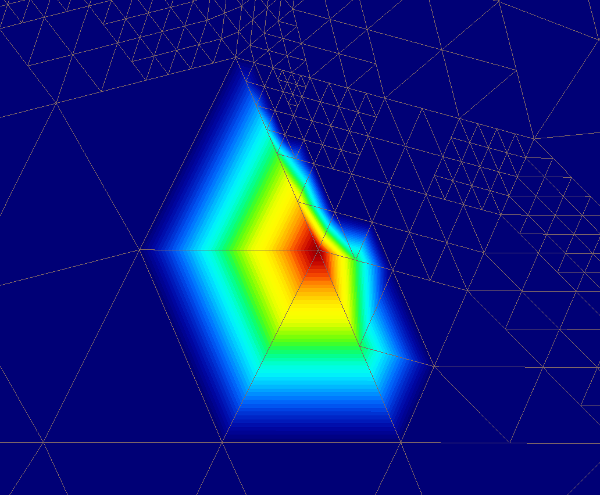
\includegraphics[width=.3\textwidth]{hanging-node.png}
			\caption{Hanging nodes in the hp-FEM mesh}	
	\end{figure}
\end{center}

\vspace{-6mm} 
\begin{itemize}
\item Irregular meshes (hanging nodes and hence following constraints spreading in the mesh).
\item \vspace{-2mm} Non-uniform polynomial order, constrained edge DOFs.
\item \vspace{-2mm} Different meshes (again for memory-demands reasons) for individual equations.
\item \vspace{-2mm} Various refinement approaches for individual refined element (h-, p-, hp-).
\end{itemize}

\end{frame}


\subsection{hp-FEM test problem solution}
\begin{frame}
\begin{center}
\includemedia[activate=onclick, width=\textwidth]{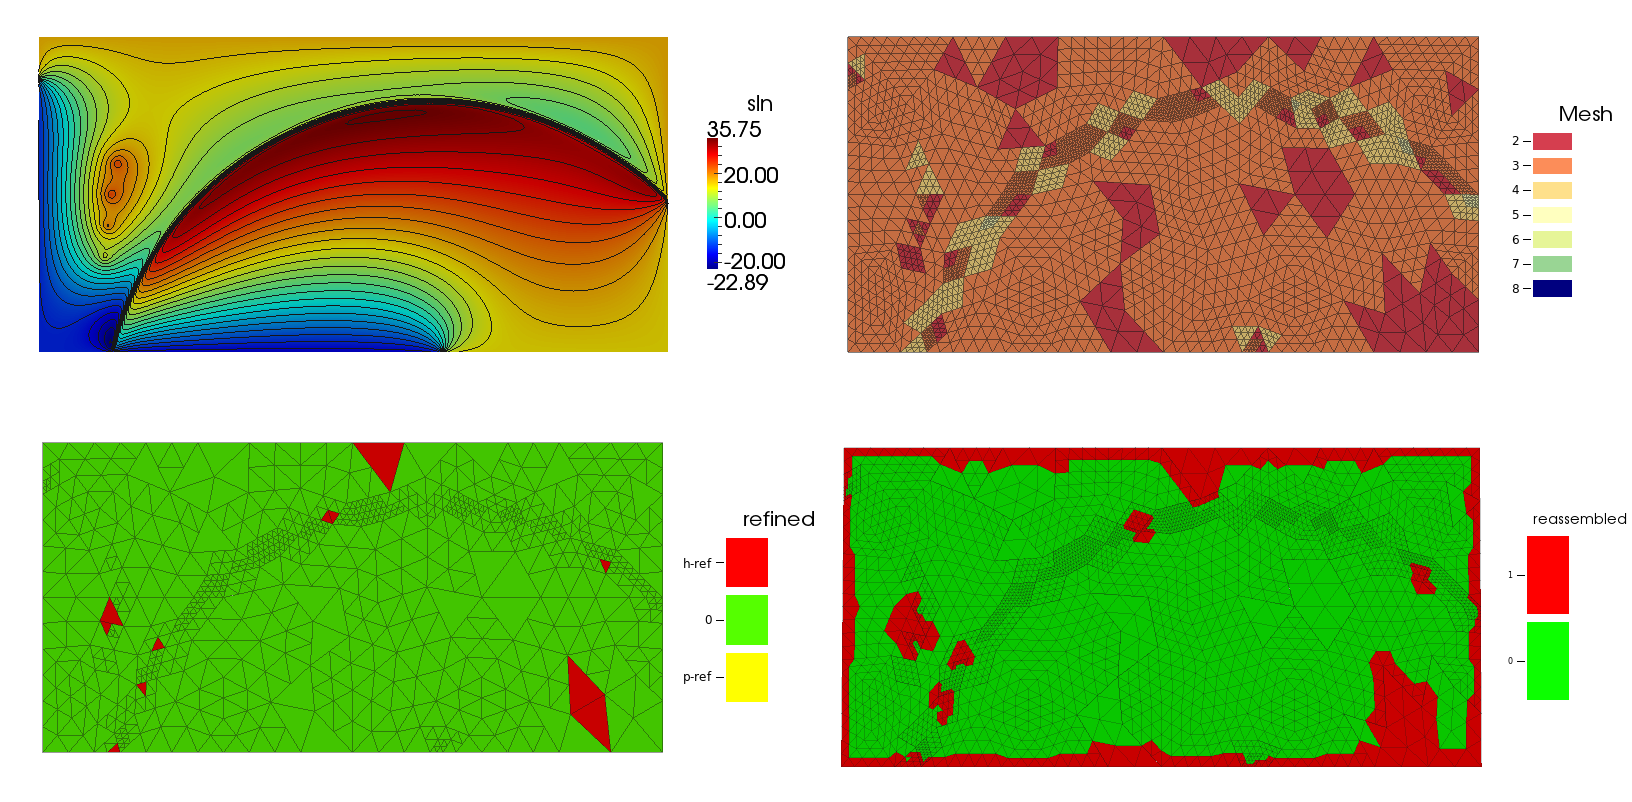
\includegraphics{40.png}}{final.swf}
\end{center}
\end{frame}

\subsection{hp-FEM meshes detail}
\begin{frame}
\begin{center}
	\begin{figure}[h!]
	\centering
	\begin{subfigure}{.6\textwidth}
		\centering
		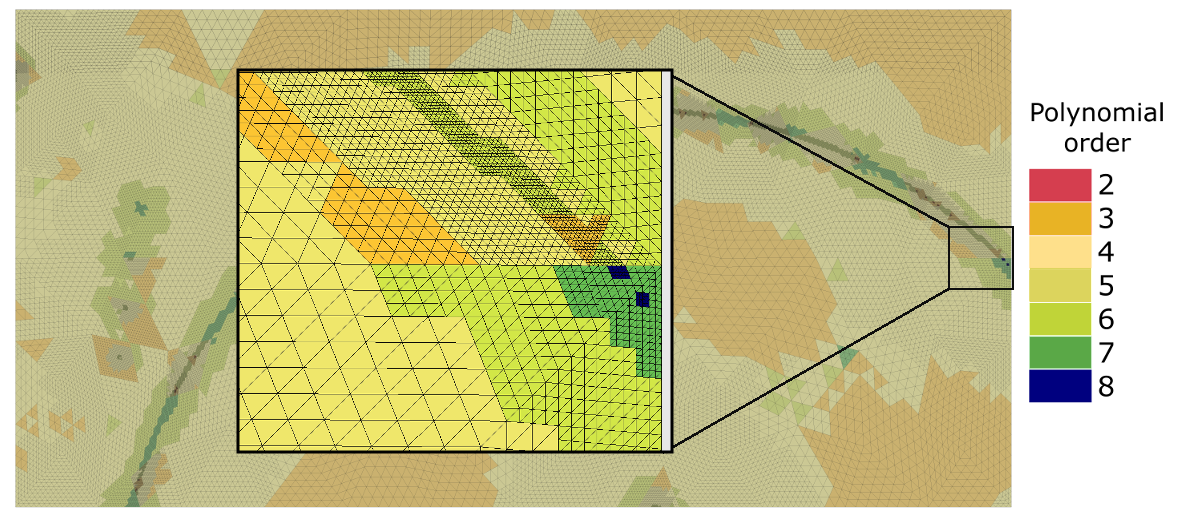
\includegraphics[width=\textwidth]{final_mesh-detail-1.png}
	\end{subfigure}
	\begin{subfigure}{.6\textwidth}
		\centering
		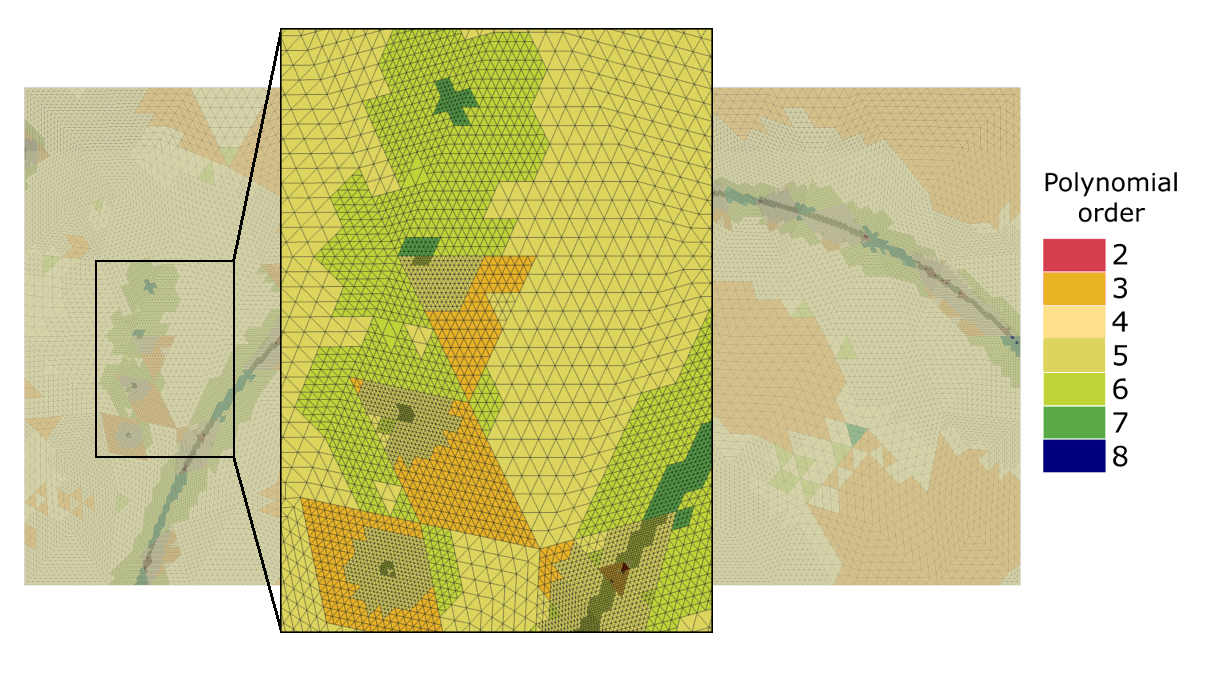
\includegraphics[width=\textwidth]{final_mesh-detail-2.png}
	\end{subfigure}
	\caption{Details of the hp-FEM mesh}
	\end{figure}
\end{center}
\end{frame}

\subsection{Data reuse background}

\begin{frame}
\begin{center}
	\begin{figure}[h!]
			\centering
			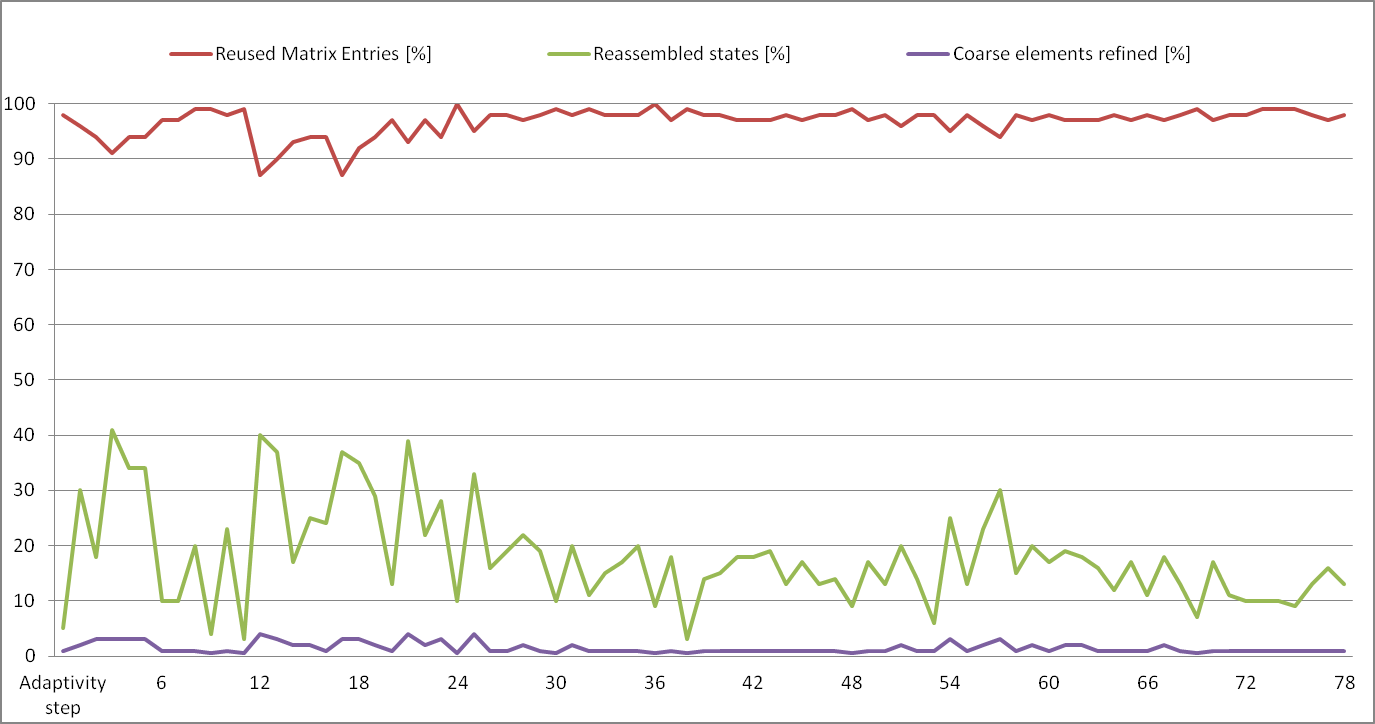
\includegraphics[width=.55\textwidth]{graf-technicky.png}
	\end{figure}
\end{center}

\vspace{-6mm} 
\begin{itemize}
\item Coarse elements refined (avg. 1.5\% per adaptivity step in this test case)
\begin{itemize}
\item \vspace{-2.5mm} The value depends on algorithm settings (higher percentage yields less steps, smaller yields mesh closer to the optimal one).
\item \vspace{-2.5mm} the reference solution adaptivity approach selects refinements of the coarse mesh,\\
\vspace{-2.5mm} these are carried out and afterwards the appropriate refinements of the reference space are done.
\end{itemize}
\item \vspace{-2mm} Reassembled states (avg. 18\% per adaptivity step in this test case)
\begin{itemize}
\item \vspace{-2.5mm} Assembling of the matrix is done based on the reference space.
\item \vspace{-2.5mm} We need to identify which reference states(=elements) we need to visit in the element-based assembling.
\end{itemize}
\item \vspace{-2mm} Reused Matrix Entries (avg. 96.7\% per adaptivity step in this test case)
\begin{itemize}
\item \vspace{-2.5mm} {\small Although we still need to visit a lot of elements(\~18\%), we only need to calculate a few matrix \% rhs entries (\~3.3\%).}
\end{itemize}

\item \vspace{-2mm} Treatment of the boundary condition is a separate issue.
\begin{itemize}
\item \vspace{-2.5mm} now the boundary is treated as a single point of recalculation:\\
\vspace{-2.5mm} (if one element with nonzero intersection with Dirichlet lift support is recalculated, all of such elements are)
\item \vspace{-2.5mm} optimization of this logic is a work-in-progress.
\end{itemize}
\end{itemize}

\end{frame}


\subsection{Mark the necessary (re-)calculations}

\begin{frame}
After Element refinement, we need to find all the matrix \& rhs entries we need to recalculate - In practice, such entries (both existing entries and new ones for the DOFs added in the last step) are marked and the algorithm copies the previous entries iff. those are not marked.

\begin{center}
	\begin{figure}[h!]
			\centering
			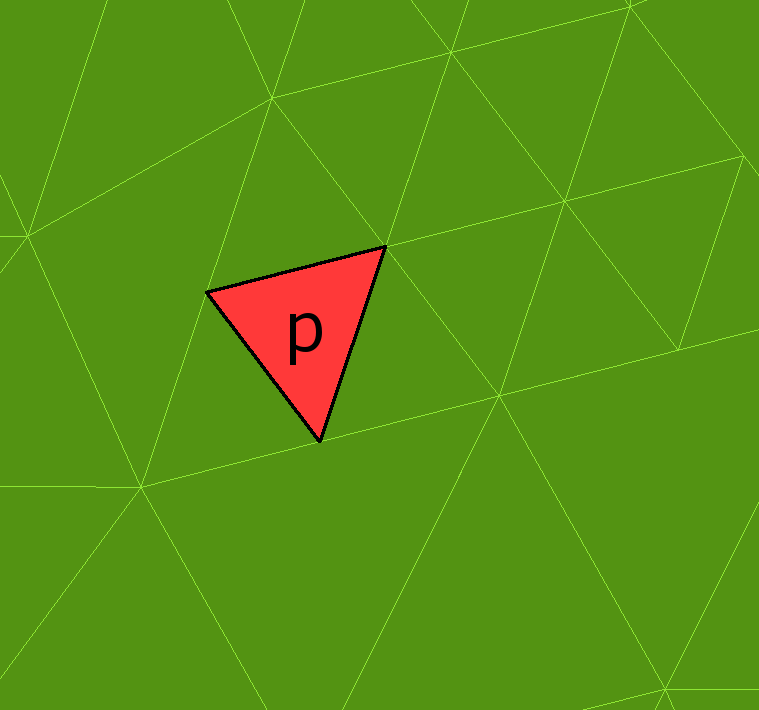
\includegraphics[width=.4\textwidth]{recalculation-1.png}
			\caption{Element with a polynomial order p is selected for refinemt - should there be a refinement only in p, it is only a simple case of the more general case of h-refinement presented here.}
	\end{figure}
\end{center}
\end{frame}

\begin{frame}
Without loss of generality, we can assume (for the sake of simplicity), that the refinement is in h only here.\ \\\ \\

\begin{center}
	\begin{figure}[h!]
			\centering
			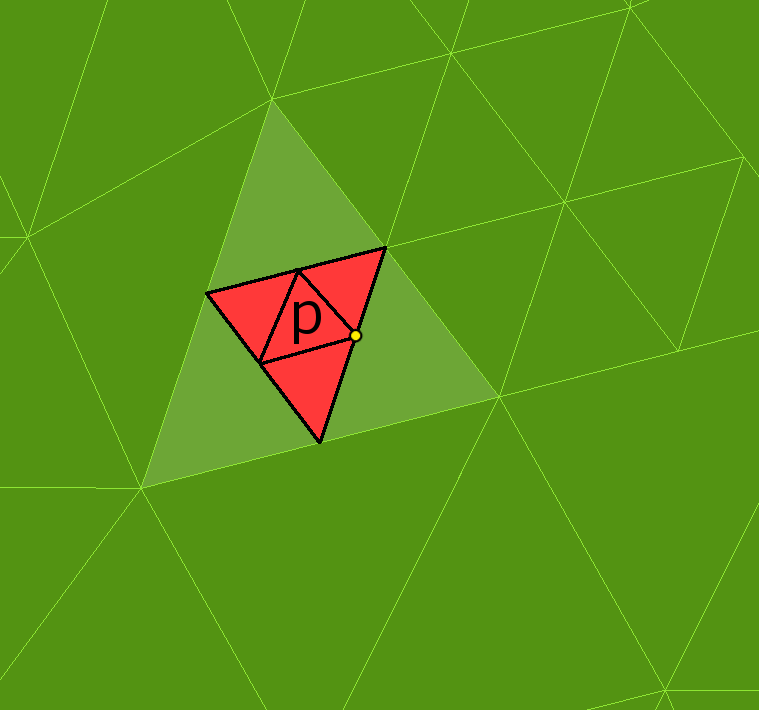
\includegraphics[width=.4\textwidth]{recalculation-2.png}
			\caption{Element is split into four equal sized sones, all with polynomial order p (all DOFs of all sons are marked). The yellow dot (constrained vertex DOF) is a place where we start our considerations about what else to mark.}
	\end{figure}
\end{center}
\end{frame}

\begin{frame}
The constrained vertex DOF is constrained by the two vertex DOFs and the edge DOF(s) displayed.\ \\
These DOFs are also marked as their overall contribution to the matrix \& rhs changed due to the element refinement.

\begin{center}
	\begin{figure}[h!]
			\centering
			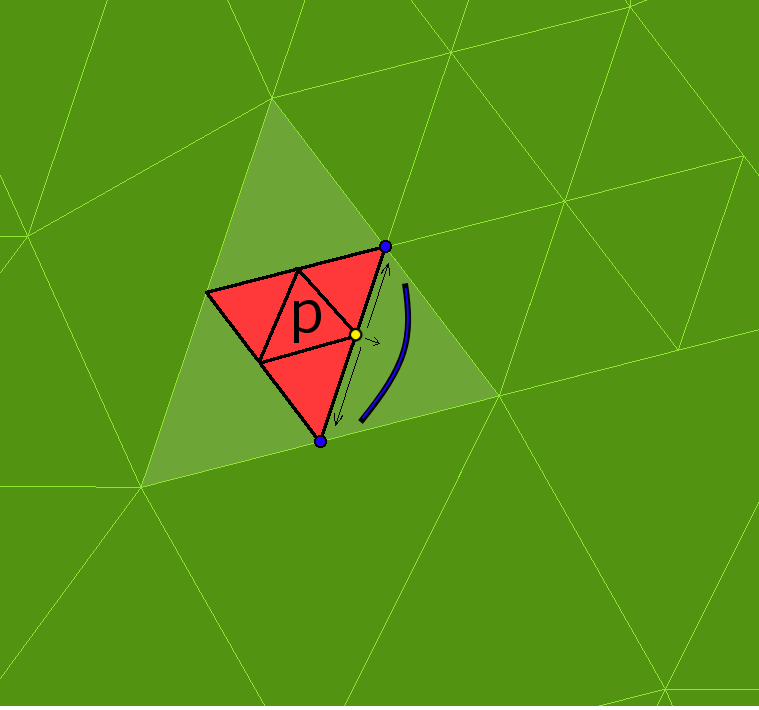
\includegraphics[width=.4\textwidth]{recalculation-3.png}
			\caption{We mark the DOF as a whole column/row in the matrix (even though we could employ marking pairs for the matrix in order to reduce recalculations - but making the algorithm for marking slower on the other hand).}
	\end{figure}
\end{center}
\end{frame}

\begin{frame}
For each of the marked DOFs, we need to visit elements where the DOF has nonempty support (these are marked in lighter color) - displayed are such elements for the top marked constraining vertex.

\begin{center}
	\begin{figure}[h!]
			\centering
			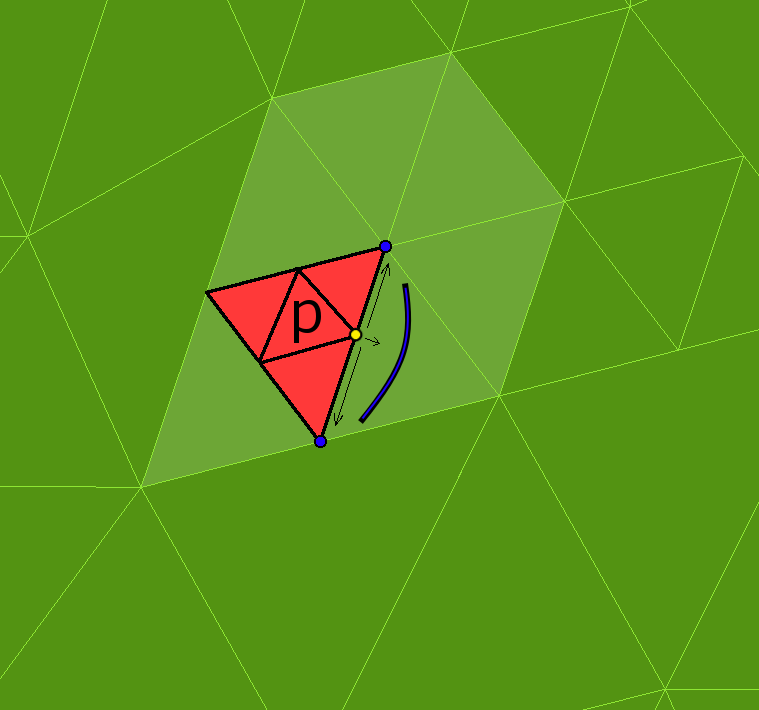
\includegraphics[width=.4\textwidth]{recalculation-4.png}
			\caption{This does not mean that the entire local stiffness matrix belonging to the adjacent will be recalculated, only the necessary (due to marking) entries in matrix \& rhs.}
	\end{figure}
\end{center}
\end{frame}

\begin{frame}
Finally we find all the elements we need to visit - one can notice here that due to the presence of hanging nodes, the algorithm to find such elements needs to be thorough.

\begin{center}
	\begin{figure}[h!]
			\centering
			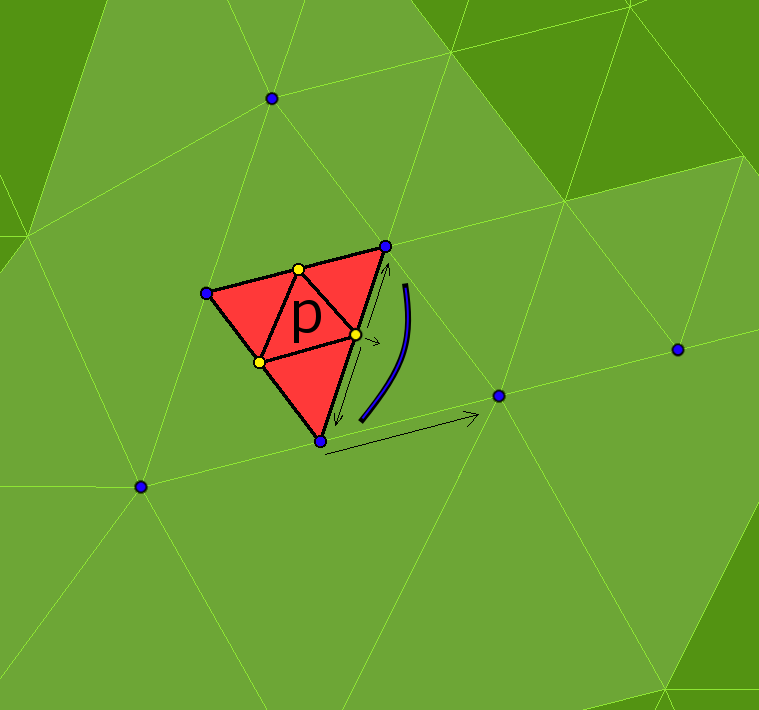
\includegraphics[width=.4\textwidth]{recalculation-5.png}
			\caption{Final set of elements we need to visit during the element-wise assembling, on which we will evaluate the marked DOFs.\ \\Note: The vertices that are responsible for spreading the dependencies over the mesh are displayed in blue.}
	\end{figure}
\end{center}
\end{frame}

\end{document}